
% This LaTeX was auto-generated from MATLAB code.
% To make changes, update the MATLAB code and republish this document.

\documentclass{article}
\usepackage{graphicx}
\usepackage{color}

\sloppy
\definecolor{lightgray}{gray}{0.5}
\setlength{\parindent}{0pt}

\begin{document}

    
    
\subsection*{Contents}

\begin{itemize}
\setlength{\itemsep}{-1ex}
   \item Density Plot
\end{itemize}
\begin{par}
Set boxes
\end{par} \vspace{1em}
\begin{verbatim}
boxLeft = 0.45;
boxRight = 0.55;
boxBottom = 0.7;
boxTop = 0.3;

Btype = 's'; % specular boxes
% Btype = 'd'; % diffusive boxes

dx = regL / nx;
dy = regW / ny;

condHigh = 1;
condLow = 10e-2;

cMap = zeros(nx,ny);

for i = 1:nx

    for j = 1:ny

        if ((i>=boxLeft*nx) && (i<=boxRight*nx) && (((j>=boxBottom*ny) && (j<=ny)) || ((j<=boxTop*ny) && (j>=0))))
            cMap(i,j) = condLow;
        else
            cMap(i,j) = condHigh;
        end

    end

end

G = sparse(nx*ny);
F = zeros(nx*ny,1);

for i = 1:nx
    for j = 1:ny

        n = j + (i-1)*ny; % node mapping

        if i == 1 % left side = V_0

            G(n,n) = 1;
            F(n) = V_0;

        elseif i == nx % right side = 0V

            G(n,n) = 1;
            F(n) = 0;

        elseif j == ny % top side = insulated

            % only three resistors:
            % n(x-1,y), n(x+1,y), n(x,y-1)

            nxm = j + (i-2)*ny;
            nxp = j + i*ny;
            nym = (j-1) + (i-1)*ny;

            rxm = (cMap(i,j) + cMap(i-1,j))/2.0;
            rxp = (cMap(i,j) + cMap(i+1,j))/2.0;
            rym = (cMap(i,j) + cMap(i,j-1))/2.0;

            G(n,n) = -(rxm + rxp + rym);
            G(n,nxm) = rxm;
            G(n,nxp) = rxp;
            G(n,nym) = rym;

        elseif j == 1 % bottom side = insulated

            % only three resistors:
            % n(x-1,y), n(x+1,y), n(x,y+1)

            nxm = j + (i-2)*ny;
            nxp = j + i*ny;
            nyp = (j+1) + (i-1)*ny;

            rxm = (cMap(i,j) + cMap(i-1,j))/2.0;
            rxp = (cMap(i,j) + cMap(i+1,j))/2.0;
            ryp = (cMap(i,j) + cMap(i,j+1))/2.0;

            G(n,n) = -(rxm + rxp + ryp);
            G(n,nxm) = rxm;
            G(n,nxp) = rxp;
            G(n,nyp) = ryp;

        else % middle node

            nxm = j + (i-2)*ny;
            nxp = j + i*ny;
            nym = (j-1) + (i-1)*ny;
            nyp = (j+1) + (i-1)*ny;

            rxm = (cMap(i,j) + cMap(i-1,j))/2.0;
            rxp = (cMap(i,j) + cMap(i+1,j))/2.0;
            rym = (cMap(i,j) + cMap(i,j-1))/2.0;
            ryp = (cMap(i,j) + cMap(i,j+1))/2.0;

            % middle nodes in G, based on the sum of four neighbour cells
            G(n,n) = -(rxm + rxp + rym + ryp);
            G(n,nxm) = rxm;
            G(n,nxp) = rxp;
            G(n,nym) = rym;
            G(n,nyp) = ryp;

        end

    end
end

V = G\F;

Vmap = zeros(nx,ny); % initialize matrix
n = 0; % clear/reset node index n

for i = 1:nx
    for j = 1:ny
        n = j + (i-1)*ny;
        Vmap(i,j) = V(n);
    end
end

Ex = [];
Ey = [];

for i = 1:nx
    for j = 1:ny

        % Calculate Ex
        if i == 1
            Ex(i,j) = Vmap(i+1,j) - Vmap(i,j);
        elseif i == nx
            Ex(i,j) = Vmap(i,j) - Vmap(i-1,j);
        else
            Ex(i,j) = (Vmap(i+1,j) - Vmap(i-1,j)) / 2.0;
        end

        % Calculate Ey
        if j == 1
            Ey(i,j) = Vmap(i,j+1) - Vmap(i,j);
        elseif j == ny
            Ey(i,j) = Vmap(i,j) - Vmap(i,j-1);
        else
            Ey(i,j) = (Vmap(i,j+1) - Vmap(i,j-1)) / 2.0;
        end

    end
end

Ex = -Ex;
Ey = -Ey;
Exy = sqrt(Ex.^2 + Ey.^2);

Jx = cMap.*Ex;
Jy = cMap.*Ey;
Jxy = sqrt(Jx.^2 + Jy.^2);

Current = mean(Jxy.*(regL*regW*10^(13)), 'all');

figure(7)
subplot(2,2,1); surf(cMap')
title('Conduction Map')
view(2) % adjust camera angle for better view

subplot(2,2,2); surf(Vmap)
title('Electrostatic Charge')
view(135,45) % adjust camera angle for better view

subplot(2,2,3); quiver(Ey,Ex)
title('Electric Field')
view(90,90) % adjust camera angle for 2D view

subplot(2,2,4); surf(Jxy')
title('Current Density')
view(135,45) % adjust camera angle for better view

xPos = regL.*rand(1,numElec); % set random initial x position
yPos = regW.*rand(1,numElec); % set random initial y position
\end{verbatim}

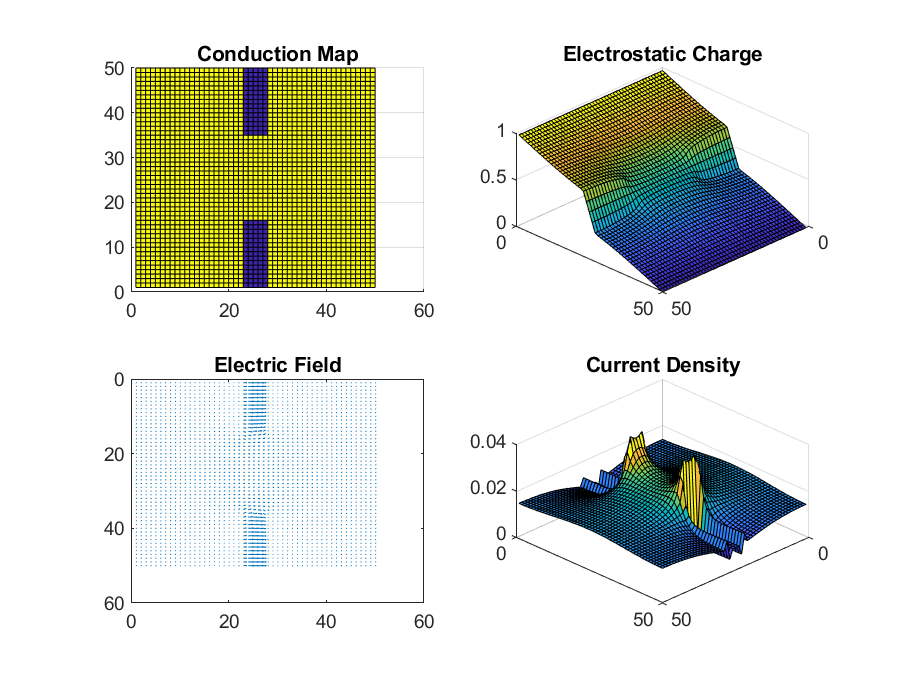
\includegraphics [width=4in]{assign3part2_01.eps}
\begin{par}
Before moving forward, we must ensure all initial positions lie outisde the boxes.
\end{par} \vspace{1em}
\begin{verbatim}
for i = 1:numElec
    while ((xPos(i)>=(boxLeft*regL)) && (xPos(i)<=(boxRight*regL))) && (((yPos(i)>=(boxBottom*regW)) || (yPos(i)<=(boxTop*regW))))
        xPos(i) = regL.*rand; % set random initial x position
        yPos(i) = regW.*rand; % set random initial y position
    end
end

% velocities will also be assigned randomly according to the
% Maxwell-Boltzmann distribution with an average of the speeds being the
% thermal velocity.

xVel = sqrt(3*kb * T/m_n)*randn(1,numElec);
yVel = sqrt(3*kb * T/m_n)*randn(1,numElec);

[Xm,Ym]= meshgrid(L,W);

% we also need to determine the probability of an electron scattering. This
% is given by the function: \[P_{scat} = 1 - e^{-dt/ \tau_{mn}}\]

Pscat = 1 - exp(-dt/t_mn);

for t = 1:numTimeStep

    figure(8)
    for n = 1:numDispElec
        plot(xPos(n), yPos(n),'.','color',Cols(n,:))
    end
    title('Electrons as Carriers in N-type Si crystal (with Collision)')
    axis([0 regL 0 regW])
    hold on
    makeBox(boxLeft,boxRight,1,boxBottom,regL,regW); % top box
    makeBox(boxLeft,boxRight,boxTop,0,regL,regW); % bottom box

    % save old x and y positions
    xPrev = xPos;
    yPrev = yPos;

    randNum = rand(1, numElec); % generate a random number for each electron
    scatter = randNum < Pscat; % determine if electron scatters
    xVel(scatter) = sqrt(3*kb * T/m_n)*randn;
    yVel(scatter) = sqrt(3*kb * T/m_n)*randn;

    % use linear interpolation to determine E-field at each electron postion
    Exp = interp2(Xm,Ym,Ex,xPos,yPos);
    Eyp = interp2(Xm,Ym,Ey,xPos,yPos);

    % calculate force on each electron
    Fx = q*Exp*10^9;
    Fy = q*Eyp*10^9;

    accelX = (Fx./m_n); % acceleration
    accelY = (Fy./m_n);

    % determine new X and Y velocities
    xVel = dt.*accelX + xVel;
    yVel = dt.*accelY + yVel;

    newXPos = xPos + xVel*dt;
    newYPos = yPos + yVel*dt;

    if Btype == 's' % specular boxes, just bounce

        for i = 1:numElec
            if ((newXPos(i)>=(boxLeft*regL)) && (newXPos(i)<=(boxRight*regL))) && (((newYPos(i)>=(boxBottom*regW)) || (newYPos(i)<=(boxTop*regW))))
                if (xPrev(i) <= boxLeft*regL) || (xPrev(i) >= boxRight*regL )
                    xVel(i) = -xVel(i);
                elseif (yPrev(i) <= boxBottom*regW) || (yPrev(i) >= boxTop*regW)
                    yVel(i) = -yVel(i);
                end
            end
        end

    elseif Btype == 'd' % diffusive boxes, re-thermalize

        for i = 1:numElec
            if ((newXPos(i)>=(boxLeft*regL)) && (newXPos(i)<=(boxRight*regL))) && (((newYPos(i)>=(boxBottom*regW)) || (newYPos(i)<=(boxTop*regW))))
                if (xPrev(i) <= boxLeft*regL) || (xPrev(i) >= boxRight*regL )
                    xVel(i) = -xVel(i);
                    yVel(i) = sqrt(3*kb * T/m_n)*randn;
                elseif (yPrev(i) <= boxBottom*regW) || (yPrev(i) >= boxTop*regW)
                    xVel(i) = sqrt(3*kb * T/m_n)*randn;
                    yVel(i) = -yVel(i);
                end
            end
        end

    end

    crossRight = newXPos >= regL;
    crossLeft = newXPos <= 0;
    xPos = xPos + xVel*dt;
    xPos(crossRight) = 0;
    xPos(crossLeft) = regL;

    crossTop = newYPos > regW;
    crossBottom = newYPos < 0;
    yVel(crossTop) = -yVel(crossTop);
    yVel(crossBottom) = -yVel(crossBottom);
    yPos = yPos + yVel*dt;

end
\end{verbatim}

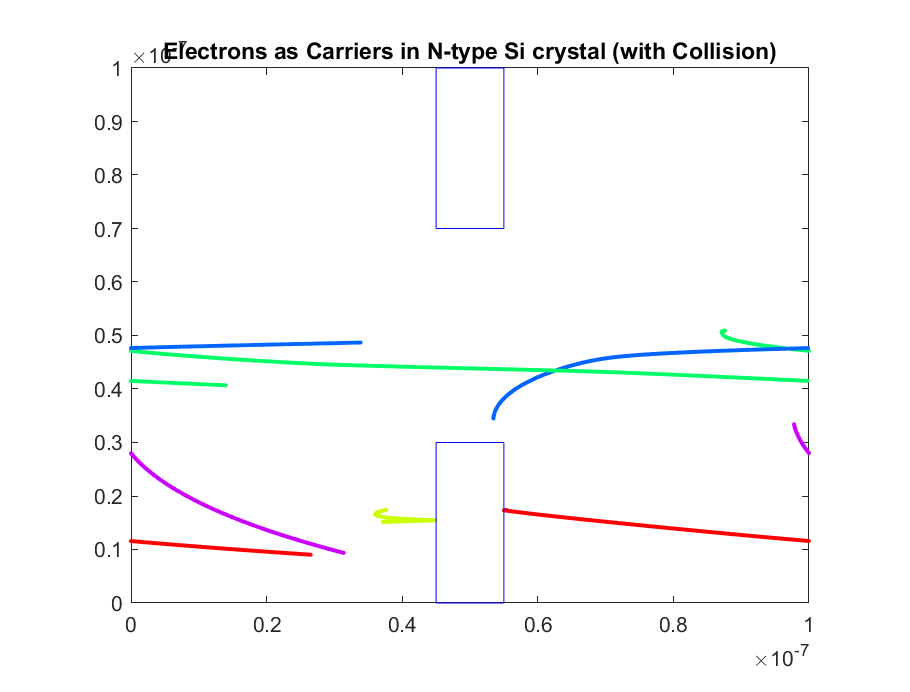
\includegraphics [width=4in]{assign3part2_02.eps}


\subsection*{Density Plot}

\begin{par}
After the completion of the simulation, we can take the final positions of the electrons and create a density plot. To do this, we divide the region into a meshgrid, loop through each differential area and count the number of electrons in that area creating a matrix of the number of electrons located in each segment of the region. This matrix can be plotted as a surface to help us visualize the electron density of the area.
\end{par} \vspace{1em}
\begin{verbatim}
% xPos and yPos now hold the final x and y positions of the electrons
% respectively. nx and ny (declared in main) are the number of segments the
% x and y directions will be divided into - thus the region will be divided
% into nx*ny smaller areas. We can divide the electrons x and y positions
% by the length and width and multiply by nx and ny respectively to obtain
% the index in which each electron resides in (these will have to be
% rounded up such that we are left with only whole integer values)

xi = ceil(xPos/regL*nx); % x index
yi = ceil(yPos/regW*ny); % y index

% loop through each smaller area and count the number of electrons present
for i = 1:nx
    for j = 1:ny

        match = (xi==i) & (yi==j); % search for all electrons at the current i,j index

        % match will have a 1 for every electron located at current index,
        % taking the sum gives the total number of electrons located at
        % this cell in the meshgrid
        sum_e = sum(match);

        densityPlot(i,j) = sum_e; % save this sum into a matrix to be mapped out

    end
end

densityPlot = densityPlot';

figure(9)
surf(densityPlot,'EdgeColor','interp')
view(2)
title('Density Plot')
\end{verbatim}

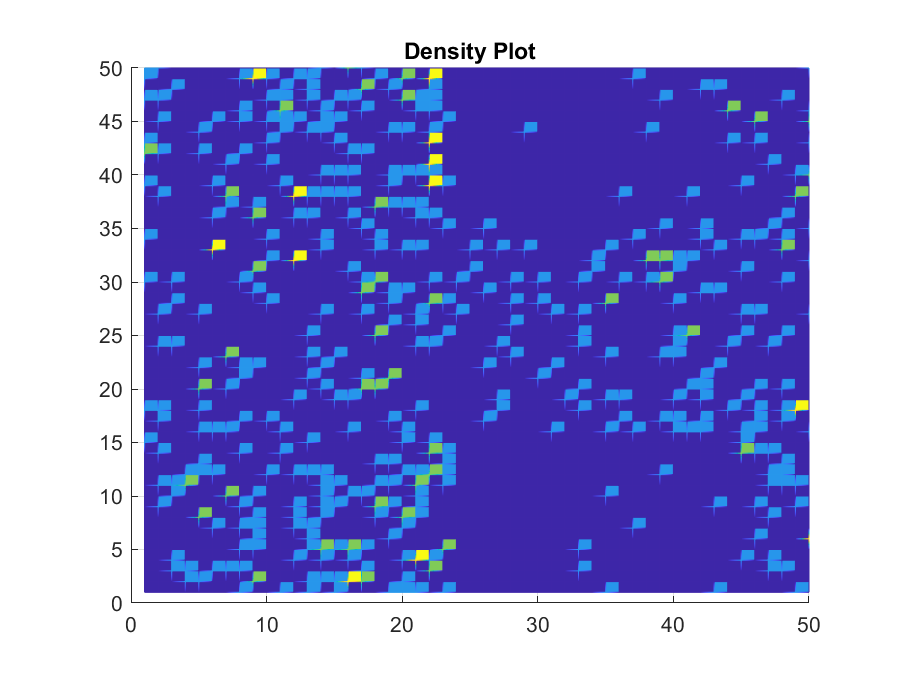
\includegraphics [width=4in]{assign3part2_03.eps}



\end{document}

